%!TEX root = ./main.tex

%%%%%%%%%%%%%%%%%%%%%%%%%%%%%%%%%%%%%%%%%%%%%%%%%%%%%%%%%%%%%%%%
%%
%% Vorlage für Bachelor Arbeit und weitere Dokumentationen (T1000 - T3300)
%%   von Maximilian Knopf
%%   inspiriert von einer DHBW Heidenheim Vorlage, https://github.com/programonaut/latex-template
%%
%% Erstellen mitteles Kommandozeile:
%%   pdflatex main.tex
%%   biber main
%%   pdflatex main.tex
%%   pdflatex main.tex
%%%%%%%%%%%%%%%%%%%%%%%%%%%%%%%%%%%%%%%%%%%%%%%%%%%%%%%%%%%%%%%%

%!TEX root = ../main.tex

%% Literatur Resourcendateien
\newcommand{\loadbibresources}{
	\bibliography{resources/quellen.bib}
}
\newcommand{\quoteStyle}{numeric-comp}						% Zitierstil: numeric-comp, alphabetic, ieee

%% Dokumententyp
%\newcommand{\documentType}{T3\_1000}				% Praxisarbeit (Semester 1 & 2)
%\newcommand{\documentType}{T3\_2000}				% Praxisarbeit (Semester 3 & 4)
%\newcommand{\documentType}{T3\_2001}				% Praxisarbeit, Teil 1 (Semester 3, Teil 1)
% \newcommand{\documentType}{T3\_2002}				% Praxisarbeit, Teil 2 (Semester 4, Teil 2)
%\newcommand{\documentType}{T3\_3000}				% Praxisarbeit (Semester 5)
\newcommand{\documentType}{T3\_3100}				% Studienarbeit (Semester 5 & 6)
% \newcommand{\documentType}{T3\_3300}				% Bachelor Arbeit (Semester 6)

%% Document settings
\newcommand{\documentAuthor}{Robert Orbach}			% Autor
\newcommand{\documentTitle}{Projekt IPLocate}					% Titel
\newcommand{\tutor}{Betreuer}		% Betreuer Ausbildungsfirma, nach DIN 5008
\newcommand{\evaluator}{Niels Riekers}				% Betreuer DHBW, nach DIN 5008
\newcommand{\documentPeriod}{März 2025 bis April 2025}	% Bearbeitungszeitraum
\newcommand{\course}{INF22A}						% DHBW Kurs
\newcommand{\matriculationNumber}{8489365}			% Autormatrikelnummer
\newcommand{\releaseDate}{1.04.2025}				% Veröffentlichungsdatum
\newcommand{\releaseLocation}{70174 Stuttgart}	% Veröffentlichungsort
\newcommand{\degree}{Bachelor of Science}		% akademischer Grad
\newcommand{\department}{Informatik}	% Fachrichtung
\newcommand{\locationUniversity}{Stuttgart}			% DHBW Standort
\newcommand{\companyName}{}			% Ausbildungsfirma Name
\newcommand{\companyLocation}{}	% Ausbildungsfirma Ort

%!TEX root = ../main.tex

%% Dokumentenklasse
\documentclass[%
    paper=a4,           % DIN A4
    12pt,               % Schriftgröße 12
    parskip=full,       % eine Zeile Absatzabstand
    oneside             % einseitig
    listof=totoc,		% alle Verzeichnisse in ToC einbinden
    bibliography=totoc,
    toc=listof,
    toc=chapterentrydotfill % ToC Punkte
]{scrreprt}             % KOMA Skript Report

%% Standard-Pakete
\usepackage{xstring}		            % für Stringvergleich
\usepackage[utf8]{inputenc}         	% Quelldateicodierung
\usepackage[T1]{fontenc}	            % Fontmap-Kodierung, diese wird von der pdflatex-Engine benötigt
\usepackage[english, ngerman]{babel}	% Sprache

%% ifDocType Befehlsdefinition
\newcommand{\ifDocType}[3]{%
	\IfStrEq{\documentType}{#1}{#2}{#3}%
}

%% Seiteneinstellungen
% Ränder
\usepackage[
    left=2.5cm,
    right=2.5cm,
    bottom=4cm,
    top=4cm
]{geometry}

\usepackage[onehalfspacing]{setspace}   % Zeilenabstand

% Schriftart
\usepackage{helvet}     % Arial like
\renewcommand{\familydefault}{\sfdefault}

% Kopf- und Fußzeile
\usepackage[headsepline=1pt, footsepline=1pt]{scrlayer-scrpage}
\renewcommand*\chapterpagestyle{scrheadings}
\pagestyle{scrheadings}
\ifDocType{T3\_3100}{%
    % kein Logo bei T3100
}{%
    \lohead{\includegraphics[height=1.5cm]{resources/images/logo-company.png}}
}
\chead{}
\rohead{
\includegraphics[height=1.6cm]{resources/images/logo-dhbw.png}}
\newcommand{\documentTypePhrase}{%
	\IfStrEqCase{\documentType}{%
		{T3\_1000}{Projektarbeit T1000}%
		{T3\_2000}{Projektarbeit T2000}%
		{T3\_2001}{Projektarbeit T2000, Teil 1}%
		{T3\_2002}{Projektarbeit T2000, Teil 2}%
		{T3\_3000}{Projektarbeit T3000}%
		{T3\_3100}{Seminararbeit}%
		{T3\_3200}{Studienarbeit}%
		{T3\_3300}{Bachelorarbeit}%
	}
}
\ifoot{\documentTypePhrase}
\cfoot{\documentAuthor}
\ofoot{Seite | \thepage}
\setlength{\marginparwidth}{2cm}

\usepackage{scrhack}    % KOMA Skript Fehlermeldung

%% Sonstige Pakete
\usepackage{todonotes}              % Todos in GROßBUCHSTABEN
\usepackage{graphicx}               % Bilder
\graphicspath{{resources/images/}}  % Standard Bilderpfad
\usepackage{subcaption}             % Mehrere Bilder/Tabllen in einer Figure
\usepackage{tikz}                   % für komplexe Bilderstellung
\usepackage{tabularx}               % Tabellen
\usepackage{pdfpages}               % PDF Dateien / Seiten
\usepackage{float}                  % Floating Darstellung
\usepackage{xcolor}                 % Farben
\usepackage{acronym}                % Abkürzungen, nur die Verwendeten: \usepackage[printonlyused]{acronym}
\usepackage{amsfonts}               % Mathematische Schriftart der American Mathematical Society
\usepackage{amsmath}                % Mathematische Schriftzeichen der American Mathematical Society
\usepackage{fancyvrb}               % [für Quelltext]
\usepackage{xurl}                   % URL Umbruch
\usepackage{pdflscape}              % Querformat
\usepackage{enumitem}               % Aufzählungsstile

%% Bibliographie
\usepackage[
	backend=biber,			% Recommended. Alternative: biblatex
	bibwarn=true,
	bibencoding=utf8,		% Wenn die .bib-Datei mit utf8 kodiert ist, sonst ascii
	sortlocale=de_DE,
	style=\quoteStyle,
]{biblatex}
\loadbibresources			% Lädt die Resourcen aus der config Datei
\newcommand{\mkbibnodate}{o\adddot J\adddot}        % o. J.
\AtEveryBibitem{\iffieldundef{year}{\restorefield{year}{\mkbibnodate}}{}}
\usepackage{csquotes}               % Zitierung mit Sprache verknüpfen

%% Querverweise und Links
\definecolor{LinkColor}{HTML}{00007A} % Farbe
\usepackage[%
    pdftitle={\documentTitle},
    pdfauthor={\documentAuthor},
    pdfsubject={\documentType},
    pdfcreator={pdflatex, LaTeX with KOMA-Script},
    pdfpagemode=UseOutlines,
    pdfdisplaydoctitle=true,
    pdflang={de},
    colorlinks = false,
	linkcolor=LinkColor,
	citecolor=LinkColor,
	filecolor=LinkColor,
	menucolor=LinkColor,
	urlcolor=LinkColor,
	linktocpage=true,
	bookmarksnumbered=true
]{hyperref}

%% Quelltext
\usepackage{listings}

\definecolor{comment}{HTML}{0A943F}
\definecolor{keyword}{HTML}{184FDB}
\definecolor{background}{HTML}{F2F2F2}
\definecolor{string}{HTML}{DB9418}
\lstset{
    backgroundcolor=\color{background},
    basicstyle=\ttfamily\footnotesize,
    breakatwhitespace=false,
    breakautoindent=true,
    breaklines=true,
    captionpos=b,
    commentstyle=\color{comment},
    keepspaces=true,
    keywordstyle=\color{keyword},
    morekeywords={var}
    numbers=left,
    numbersep=1em,
    numberstyle=\tiny,
    postbreak=\space,
    showspaces=false,
    showstringspaces=false,
    showtabs=false,
    stepnumber=1,
    stringstyle=\color{string},
    tabsize=2,
}


\newcommand\YAMLcolonstyle{\color{red}\mdseries}
\newcommand\YAMLkeystyle{\color{black}\bfseries}
\newcommand\YAMLvaluestyle{\color{blue}\mdseries}

\makeatletter

% here is a macro expanding to the name of the language
% (handy if you decide to change it further down the road)
\newcommand\language@yaml{yaml}

\expandafter\expandafter\expandafter\lstdefinelanguage
\expandafter{\language@yaml}
{
  keywords={true,false,null,y,n},
  keywordstyle=\color{darkgray}\bfseries,
  basicstyle=\YAMLkeystyle,                                 % assuming a key comes first
  sensitive=false,
  comment=[l]{\#},
  morecomment=[s]{/*}{*/},
  commentstyle=\color{purple}\ttfamily,
  stringstyle=\YAMLvaluestyle\ttfamily,
  moredelim=[l][\color{orange}]{\&},
  moredelim=[l][\color{magenta}]{*},
  moredelim=**[il][\YAMLcolonstyle{:}\YAMLvaluestyle]{:},   % switch to value style at :
  morestring=[b]',
  morestring=[b]",
  literate =    {---}{{\ProcessThreeDashes}}3
                {>}{{\textcolor{red}\textgreater}}1     
                {|}{{\textcolor{red}\textbar}}1 
                {\ -\ }{{\mdseries\ -\ }}3,
}

% switch to key style at EOL
\lst@AddToHook{EveryLine}{\ifx\lst@language\language@yaml\YAMLkeystyle\fi}
\makeatother

\newcommand\ProcessThreeDashes{\llap{\color{cyan}\mdseries-{-}-}}


\lstloadlanguages{PHP, Python, Java, C, C++, Bash, SQL}
\renewcommand\lstlistingname{Skript}
\renewcommand\lstlistlistingname{Skriptverzeichnis}
\def\lstlistingautorefname{Skript}

%% Chapter Style
\definecolor{chapterBlue}{RGB}{47,84,150}
\addtokomafont{chapter}{\color{chapterBlue}}
\addtokomafont{section}{\color{chapterBlue}}
\addtokomafont{subsection}{\color{chapterBlue}}
\addtokomafont{subsubsection}{\color{chapterBlue}}
\RedeclareSectionCommand[beforeskip=0pt,afterindent=false,afterskip=1em]{chapter}
\RedeclareSectionCommand[beforeskip=0pt,afterindent=false,afterskip=1em]{section}
\RedeclareSectionCommand[beforeskip=0pt,afterindent=false,afterskip=1em]{subsection}
\RedeclareSectionCommand[beforeskip=0pt,afterindent=false,afterskip=1em]{subsubsection}

%% Caption Style (Bsp.: Bilderunterschrift)
\addtokomafont{caption}{\small}

%% Cover Einstellungen
\title{\documentTitle}
\author{\documentAuthor}
\date{\releaseDate}


%% Start des Dokuments
\begin{document}
    %TODO: Liste aller TODOs, auskommentieren für die Abgabe!
    % \listoftodos

    %% Titelblatt
    %!TEX root = ../main.tex

\begin{titlepage}
%% DHBW_Logo
\begin{tikzpicture}[remember picture, overlay]
	\node[anchor=north east,inner xsep=50pt, inner ysep=25pt] at (current page.north east)
	{
\includegraphics[height=2cm]{resources/images/logo-dhbw}};
\end{tikzpicture}

%% Firmen Logo
\ifDocType{T3\_3100}{%
	% kein Logo bei T3100
}{%
	\begin{tikzpicture}[remember picture, overlay]
		\node[anchor=north west,inner xsep=50pt, inner ysep=25pt] at (current page.north west)
		{\includegraphics[height=2cm]{resources/images/logo-company}};
	\end{tikzpicture}
}

\enlargethispage{20mm}
\begin{center}
	\vspace*{0mm}	{\LARGE\textbf{\documentTitle}}\\
	\vspace*{12mm}
	\vspace*{12mm}	{\large\textbf{\documentTypePhrase}}\\

	\ifDocType{T3\_3300}{
		\vspace*{12mm}	{für die Prüfung zum}\\
		\vspace*{3mm}	{\degree}\\
	}

	\vspace*{12mm}  {im Studiengang \department}\\
	\vspace*{3mm}  {an der Dualen Hochschule Baden-Württemberg}\\
	\vspace*{3mm}  {\locationUniversity}\\
	\vspace*{12mm}  {von}\\
	\vspace*{3mm}  {\textbf{\documentAuthor}}\\
	\vspace*{12mm}  {\releaseDate}\\
\end{center}

\vfill

\begin{spacing}{1.2}
	\begin{tabbing}
		mmmmmmmmmmmmmmmmmmmmmmmmmm \= \kill
		\textbf{Bearbeitungszeitraum} \> \documentPeriod \\
		\textbf{Matrikelnummer, Kurs} \> \matriculationNumber, \course \\
		\ifDocType{T3\_3100}{%
			% keine Firma bei T3100
			\textbf{Bei Dozent} \> \evaluator
		}{%
			\textbf{Dualer Partner} \> \companyName, \companyLocation \\
			\textbf{Betreuer des Dualen Partners} \> \tutor \\
		}%
		\ifDocType{T3\_3300}{%
			% DHBW Gutachter 
			\textbf{Gutachter der DHBW \locationUniversity} \> \evaluator
		}{}
	\end{tabbing}
\end{spacing}
\end{titlepage}


    \pagestyle{scrheadings}
    \pagenumbering{Roman}

    %% Sperrvermerk
    \ifDocType{T3\_3100}{%
            % kein Sperrvermerk für T3100
        }{%
            %!TEX root = ../main.tex

\chapter*{Sperrvermerk}
Der Inhalt dieser Arbeit darf weder als Ganzes noch in Auszügen Personen außerhalb des Prüfungsprozesses und des Evaluationsverfahrens zugänglich gemacht werden, sofern keine anderslautende Genehmigung der Ausbildungsstätte vorliegt.

% Source: https://www.dhbw-stuttgart.de/studierendenportal/horb/elektrotechnik/studienbetrieb/praxisarbeiten/ [04.2022]

        }%

    %% Erklärung
    %!TEX root = ../main.tex



    %% Abstract
    % %!TEX root = ../main.tex

\chapter{Abstract}
Aktivierungsfunktionen sind essenziell für die Leistungsfähigkeit neuronaler Netzwerke, da sie Nichtlinearitäten einführen und die Verarbeitung komplexer Muster ermöglichen. Diese Arbeit untersucht zwei prominente Aktivierungsfunktionen: Sigmoid und ReLU. Ziel ist es, ihre Eigenschaften und ihr Verhalten in verschiedenen Szenarien des maschinellen Lernens systematisch zu vergleichen. Der Fokus liegt dabei auf zentralen Attributen wie Trainingsgeschwindigkeit, Genauigkeit (Accuracy), Präzision, Verhalten bei Gradientenproblemen und Rechenaufwand.
Die Untersuchung zeigt, dass ReLU durch die Einfachheit und Effizienz in vielen modernen Anwendungen die bevorzugte Wahl ist, insbesondere in DNNs, die von Problemen wie dem Vanishing Gradient betroffen sind. Sigmoid weist, trotz der eingeschränkten Verwendung in heutigen Architekturen, Stärken in spezifischen Anwendungsbereichen auf, die näher beleuchtet werden.
Die Ergebnisse dieser Arbeit liefern eine fundierte Grundlage für die Wahl der Aktivierungsfunktion in maschinellen Lernsystemen und verdeutlichen die entscheidende Rolle, die diese für die Leistungsfähigkeit und Effizienz neuronaler Netzwerke spielt.

\textit{
Activation functions are essential for the performance of neural networks as they introduce non-linearities and enable the processing of complex patterns. This study examines two prominent activation functions: Sigmoid and ReLU. The aim is to systematically compare their properties and behavior across various machine learning scenarios. The focus is on key attributes such as training speed, accuracy, precision, behavior in gradient-related issues, and computational cost.
The analysis shows that ReLU is the preferred choice in many modern applications due to its simplicity and efficiency, especially in deep neural networks (DNNs) affected by challenges like the vanishing gradient problem. Despite its limited use in contemporary architectures, Sigmoid demonstrates strengths in specific application areas, which are explored in detail.
The findings of this study provide a solid foundation for selecting activation functions in machine learning systems and highlight their critical role in determining the performance and efficiency of neural networks.
}






    %% Inhaltsverzeichnis
    \begin{spacing}{1.2}
        \begingroup
            \setcounter{tocdepth}{2} % subchapter Anzeigetiefe
            \tableofcontents
        \endgroup
    \end{spacing}

    \clearpage
    \pagenumbering{arabic}

    % Abkürzungsverezeichnis
    % %!TEX root = ../main.tex

\addchap{Abkürzungsverzeichnis}

\begin{acronym} %[ABCDEF]               % längste Abkürzung
	%\setlength{\itemsep}{-\parsep}     % Kein Abstand, kompakte Darstellung
	% Sortiere von Hand oder automatisch mit Kommandozeile (windows): sort file.txt /O file.txt

	\acro{t-SNE}{t-distributed Stochastic Neighbor Embedding}
	\acro{PCA}{Principal Component Analysis}

\end{acronym}


    % \acresetall

    %% Inhalt
    %!TEX root = ../main.tex

\chapter{Einleitung}
Cloud Computing hat sich in den letzten Jahren zu einem zentralen Bestandteil moderner IT-Infrastrukturen entwickelt. Unternehmen nutzen Cloud-Dienste, um ihre Anwendungen effizienter zu betreiben, Kosten zu senken und die Skalierbarkeit zu verbessern. 

Im Rahmen der Vorlesung haben wir das Themenfeld erkundet und uns mit den Möglichkeiten und Herausforderungen von Cloud Computing auseinandergesetzt. Um diese selbst auszuprobieren, haben wir die Chance, ein eigenes Projekt unter anwendung der Möglichkeiten des Coud Computing zu realisieren.

In diesem Projekt wurde eine Webanwendung unter Nutzung von Cloud Computing Ansätzen entwickelt, die dem Nutzer erlaubt von IP Adressen auf die ungefähre geographische Lage zu schließen.

\chapter{Theorie}
\section{Was ist Cloud Computing?}
Klassische IT-Infrastrukturen basieren auf physischen Servern und Rechenzentren, die vor Ort betrieben werden. Da diese jedoch oft teuer zu betreiben und schwer zu skalieren sind, setzen viele Unternehmen auf Cloud Computing.

Cloud Computing bezeichnet die Bereitstellung von IT-Ressourcen wie Servern, Speicher, Datenbanken, Netzwerken und Software über das Internet. Es gibt drei Hauptmodelle:
\begin{itemize}
    \item \textbf{Infrastructure as a Service (IaaS):} Bereitstellung von virtuellen Maschinen, Netzwerken und Speicher. Der Nutzer verwaltet die Infrastruktur selbst. Beispiele: AWS EC2, Azure Virtual Machines.
    \item \textbf{Platform as a Service (PaaS):} Bereitstellung einer Plattform für die Entwicklung und Bereitstellung von Anwendungen. Der Anbieter verwaltet die Infrastruktur, während der Nutzer sich auf die Anwendung konzentriert. Beispiele: Azure App Service, Google App Engine.
    \item \textbf{Software as a Service (SaaS):} Bereitstellung von Software über das Internet. Der Nutzer verwendet die Software, ohne sich um die Infrastruktur oder Plattform kümmern zu müssen. Beispiele: Google Workspace, Microsoft Office 365.
\end{itemize}

\begin{figure}[H]
    \centering
    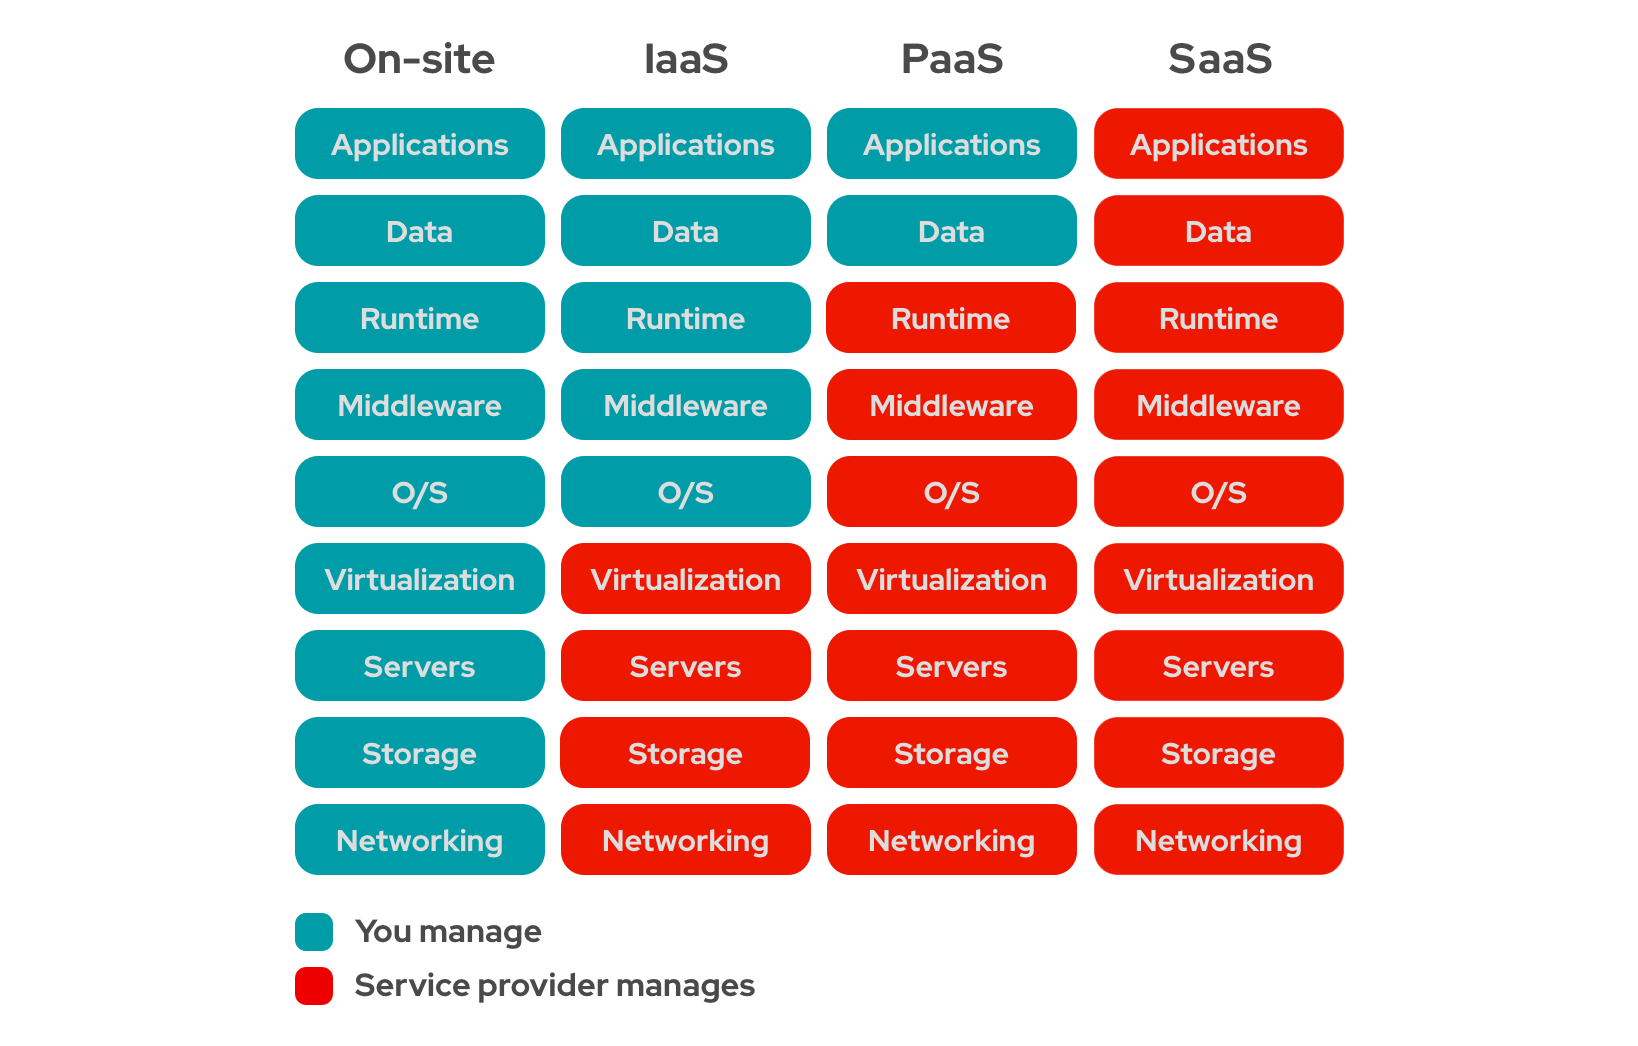
\includegraphics[width=0.8\textwidth]{resources/images/cloudcomputingtiers.png}
    \caption{Cloud Computing Modelle}
\end{figure}

\section{Warum Cloud Computing?}
Die Cloud bietet zahlreiche Vorteile:
\begin{itemize}
    \item \textbf{Skalierbarkeit:} Ressourcen können je nach Bedarf dynamisch angepasst werden.
    \item \textbf{Kostenersparnis:} Keine Investitionen in physische Hardware, Bezahlung nach Nutzung.
    \item \textbf{Flexibilität:} Zugriff auf Ressourcen von überall.
    \item \textbf{Automatisierung:} Tools wie Terraform und Ansible ermöglichen die einfache Verwaltung und Bereitstellung von Infrastruktur.
\end{itemize}

Jedoch gibt es Nachteile bei der Nutzung von Cloud Computing:
\begin{itemize}
    \item \textbf{Abhängigkeit:} Unternehmen sind von Cloud-Anbietern abhängig.
    \item \textbf{Sicherheit:} Schutz sensibler Daten und Zugriffskontrolle sind kritisch.
    \item \textbf{Kosten:} Fehlende Kontrolle über die Ressourcennutzung kann zu hohen Kosten führen.
\end{itemize}

\section{Terraform}
Terraform ist ein Open-Source-Tool zur Infrastrukturautomatisierung. Es ermöglicht die deklarative Beschreibung von Infrastruktur als Code (IaC). Mit Terraform können Ressourcen wie virtuelle Maschinen, Netzwerke und Datenbanken in verschiedenen Cloud-Anbietern wie AWS, Azure oder Google Cloud bereitgestellt werden. 

Vorteile von Terraform:
\begin{itemize}
    \item Plattformunabhängigkeit.
    \item Wiederholbare und konsistente Bereitstellung.
    \item Versionskontrolle der Infrastruktur.
\end{itemize}

\section{Ansible}
Ansible ist ein Open-Source-Tool zur Konfigurationsverwaltung und Automatisierung. Es wird verwendet, um Software zu installieren, Konfigurationen zu ändern und Anwendungen bereitzustellen.

Folgende Features machen Ansible attraktiv:
\begin{itemize}
    \item Agentenlos: Es benötigt keine zusätzliche Software auf den Zielsystemen.
    \item Einfachheit: Konfigurationen werden in YAML geschrieben.
    \item Skalierbarkeit: Kann große Umgebungen effizient verwalten.
\end{itemize}

\chapter{Umsetzung}

\section{Architektur}
Die Architektur des Projekts umfasst folgende Komponenten:
\begin{enumerate}
    \item \textbf{Virtuelles Netzwerk:} Ein Azure Virtual Network mit Subnetzen für die Anwendung und die Datenbank.
    \item \textbf{Datenbank:} Eine PostgreSQL Flexible Server Instanz, die als PaaS-Dienst bereitgestellt wird.
    \item \textbf{Webanwendung:} Mehrere virtuelle Maschinen (VMs) mit einer Load Balancer-Konfiguration, die eine Next.js-Anwendung hosten.
    \item \textbf{Monitoring:} Eine Monitoring Instanz über die mittels pgAdmin, Prometheus und Graphana die Überwachung der Anwendung erfolgt.
    \item \textbf{Automatisierung:} Terraform wird verwendet, um die Infrastruktur zu erstellen, und Ansible, um die VMs zu konfigurieren und die Anwendung bereitzustellen.
\end{enumerate}

\begin{figure}[H]
    \centering
    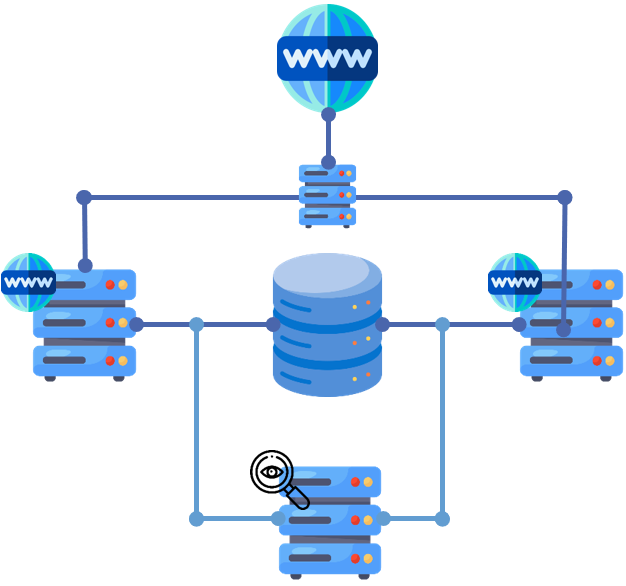
\includegraphics[width=0.8\textwidth]{resources/images/Architektur.png}
    \caption{Architektur des Projekts}
\end{figure}

\section{Aufbauablauf}

\subsection{Schritt 1: Infrastruktur mit Terraform}
Zuerst müssen die netzwerke und Server mit Terraform erstellt werden. Hierzu wird ein Azure Resource Group erstellt, in der die Ressourcen gruppiert werden. Anschließend wird ein Virtual Network mit Subnetzen für die Anwendung und die Datenbank erstellt. Danach wird eine PostgreSQL Flexible Server Instanz mit privatem Netzwerkzugriff bereitgestellt. Daruf werden zwei VMs für die Webanwendung erstellt und ein Load Balancer konfiguriert. Abchsließend wird ein Monitoring Server erstellt.

\subsection{Schritt 2: Konfiguration mit Ansible}
Konfiguration der App VMs
\begin{itemize}
    \item Installation von Node.js und PostgreSQL-Client auf den VMs.
    \item Bereitstellung der Next.js-Anwendung aus einem Git-Repository.
    \item Konfiguration der Umgebungsvariablen für die Datenbankverbindung.
    \item Erstellung eines Systemd-Dienstes, um die Anwendung automatisch zu starten.
\end{itemize}

Konfiguration des Monitoring Servers
\begin{itemize}
    \item Installation von pgAdmin, Prometheus und Grafana auf dem Monitoring Server.
    \item Konfiguration von pgAdmin zur Verwaltung der Datenbank.
    \item Konfiguration von Prometheus und Grafana zur Überwachung der Anwendung.
    \item Einrichtung von Dashboards in Grafana zur Visualisierung der Metriken.
\end{itemize}


\chapter{Fazit}
\section{Wann ist die Lösung sinnvoll?}
Die gewählte Lösung ist besonders geeignet für:
\begin{itemize}
    \item Anwendungen, die eine hohe Skalierbarkeit und Verfügbarkeit erfordern.
    \item Projekte, die von der Automatisierung der Infrastruktur profitieren.
    \item Teams, die eine konsistente und wiederholbare Bereitstellung benötigen.
\end{itemize}

\section{Was ist der Aufwand?}
Der Aufwand für die Implementierung der Lösung umfasst:
\begin{itemize}
    \item \textbf{Initiale Einrichtung:} Die Erstellung der Terraform- und Ansible-Skripte erfordert Zeit und Fachwissen.
    \item \textbf{Wartung:} Änderungen an der Infrastruktur oder der Anwendung können einfach durch Anpassung der Skripte vorgenommen werden.
    \item \textbf{Kosten:} Die Nutzung von Cloud-Diensten ist abhängig von der Ressourcennutzung und kann bei falscher Planung teuer werden.
\end{itemize}

\section{Vorteile der Lösung}
\begin{itemize}
    \item Automatisierung reduziert menschliche Fehler.
    \item Skalierbarkeit und Flexibilität der Cloud-Dienste.
    \item Sicherheit durch private Netzwerke und SSL-Verbindungen.
\end{itemize}

\section{Nachteile der Lösung}
\begin{itemize}
    \item Abhängigkeit von Cloud-Anbietern.
    \item Komplexität bei der initialen Einrichtung.
    \item Laufende Kosten für die Cloud-Dienste.
\end{itemize}

\chapter{Zusammenfassung}
Das Projekt zeigt, wie moderne Cloud-Technologien wie Terraform und Ansible genutzt werden können, um eine skalierbare und sichere Infrastruktur für eine Webanwendung bereitzustellen. Die Kombination aus IaaS und PaaS ermöglicht eine effiziente Nutzung der Cloud-Ressourcen, während die Automatisierung die Verwaltung vereinfacht. Die Lösung ist ideal für Anwendungen, die hohe Verfügbarkeit und Flexibilität erfordern, und bietet eine solide Grundlage für zukünftige Erweiterungen.
% \input{content/31_Vergleich}
% \input{content/40_Ausblick}

    %% Literaturverzeichnis
    \printbibliography[title=Literaturverzeichnis]
    \clearpage

    %% Notebook als Anhang anhängen
    % % Anhängen des Notebooks
\appendix

% \chapter{Anhang}
% %% py script anhängen
% \section{Exportiertes Notebook als Python-Script}
% \lstinputlisting[
%     language=Python, 
%     caption={Exportiertes Notebook}, 
%     label={lst:python_script}, 
%     basicstyle=\tiny, 
% ]{../notebook_als_py_script.py}

\end{document}
